\documentclass[a4paper]{article}

\usepackage{fontspec}
\usepackage{mathpazo}
\setmainfont
     [ BoldFont       = texgyrepagella-bold.otf ,
       ItalicFont     = texgyrepagella-italic.otf ,
       BoldItalicFont = texgyrepagella-bolditalic.otf ]
     {texgyrepagella-regular.otf}
\setmainfont{Gill Sans MT}

\usepackage[english]{babel}
\usepackage[utf8]{inputenc}
\usepackage{amsmath}
\usepackage{graphicx}
\usepackage[colorinlistoftodos]{todonotes}
\usepackage{physics}

%\DeclareMathOperator{\Tr}{Tr}

\title{Stochastic Reachability with Gaussian Noise}

\author{David McPherson}

\date{\today}

\begin{document}
\maketitle

\section{Introduction}
Reachability has become a valuable tool for analyzing the safety of complex dynamic systems.
Classic reachability formulates the disturbance as playing a dynamic game, wherein the disturbance aggressively chooses the worst possible choice to push the control to its limits.
By working in this worst-case scenario, we can effectively certify safety.
However, such worst case estimates for safety are often too conservative.
The agressive disturbance always fills the void for some uncertain parameter that we at least have bounds on.
However, in many cases we have more than just bounds on the disturbance.
Oftentimes we have some statistical information on the distribution of the disturbance.
Rather than throw away this distributional information, it would be ideal if we could incorporate it.

This is the idea behind stochastic reachability.
Instead of providing 100\% certain guarantees that some region is safe, it provides likelihoods of that inital state staying safe.
It effectively mixes in the doubt inherent in the disturbance's uncertainty, without making assumptions about the worst-case.

The downside is that stochastic analysis is complex.
Good computational methods for analyzing the differential games for classic reachability exist.
However, the computational methods needed for analyzing stochastic differential equations with disturbances drawn from arbitrary distributions just aren't there yet.

This work is an introduction to the world of stochastic reachability, and allowed me to begin sampling the plethora of topics required to make stochastic analysis work.
Instead of analyzing reachability for arbitrary probabilistic disturbances, I focus on disturbances that are normally distributed.
Although this is a very narrow subset of all stochastic reachability problems, I feel it is the most interesting narrow subset.

\section{Problem Statement and Motivation}
We focus on problems of the form:

\begin{equation}
  \dot{x} = f(x) + g(x) u + (\mu(x) + \sigma(x) w_t)
\end{equation}

This system is control-affine in the deterministic component with additive white Gaussian nonise with state-dependent mean $\mu(x)$ and variance $\sigma(x)$.

We are inspired to pursue problems of this form to build on work by Akametalu, Fisac, et. al \cite{KeneJaime}.
In their work, they used a Gaussian Process regression to estimate unknown disturbance forces in their system.
They then used $\mu(x) +/- 2 \sigma(x)$ as state varying bounds on the disturbance, rendering their problem into the differential game form applicable to classic reachability.
However, there is a wealth of information in the actual Gaussian distribution which represents the uncertainty in the estimate $\mu(x)$ by the variance $\sigma(x)^2$.
Our stochastic reachability formulation will allow us to leverage the full richness of the information gathered through the Gaussian process regression.

Gaussian regression can be used to estimate unknown parameters or phenomenon in a wide range of applications.
This reachability formulation can be used to provide probabilistic estimates of initial states' safety by mixing in the uncertainty measures provided in the GP's variance.

Finally, additive White noise is the go-to model for probabilistic research.
The world of applications is rich in uses for Gaussian distributions.
I hope to be able to apply this reachability framework to apply to these as well.

\section{Previous Work}
Just as deterministic reachability is intertwined with optimal control, stochastic reachability is intertwined with stochastic optimal control.
Work like Bertsekas and Shreve \cite{Bertsekas} lays a solid foundation for analyzing stochastic optimal control with discrete time.
Abate et. al \cite{AbateStoch} picks up these tools for stochastic optimal control and applies it to the hybrid reachability control problem.
We will carry the mantle of this research a little further by starting to peer at the particularly useful problem described in our Motivation.

To do so, we must analyze continuous time evolution of a stochastic system with Gaussian noise.
Here we tap into the venerable heritage of probability theory and stochastic calculus.
The study of stochastic differential systems is immense.
Here we lean heavily on the insights afforded in Evans' textbook on SDEs\cite{EvansSDE}.

All this analysis is towards the goal of molding this problem into a form acceptable to the powerful Level Set Toolbox created by Mitchell \cite{MitchellToolbox}.
By casting our problem as a Hamilton-Jacobi partial differential equation, we can leverage advances in solving these uniquely useful equations.
It is worth noting that Mitchell \cite{MitchellToolbox} actually contains an example of a stochastic differential system with white Gaussian noise, just as we are investigating.
This work expounds upon the formulation Mitchell obtained.
Where Mitchell simply pointed to Evans \cite{EvansSDE} and left out the derivation for his formula, we provide a rough derivation.
We also apply this formulation to reachability, which Mitchell does not.

\section{Derivations}
We are investigating systems with control-affine deterministic dynamics with additive white Gaussian noise.
The continuous dynamics are written as:

\begin{align}
\dot{x} = f(x) + g(x) u + (\mu(x) + \sigma(x) w_t)
\end{align}

where $w_t$ at time $t$ is sampled from a standard Gaussian distribution ($\mu = 0$ , $\sigma = 1$).
Each random variable $w_t$ is independent and identically distributed throughout all time $t$.
$w_t$ can be interpreted as a white Gaussian noise process over time.
Note that our system dynamics are described by a stochastic differential equation, rather than the typical deterministic differential equation.

\subsection{Discrete-Time Approximation}
For the sake of derivations, we will be analyzing a discrete approximation of this continuous system and then take the limit as $\Delta t$ goes to zero.
For a more rigorous, strictly continuous treatment of stochastic differential equations with additive white noise see Evans \cite{EvansSDE}.
The mathematical treatment covered here is for intuition and understanding only.

The discrete approximation to our system is:

\begin{align}
x_{k+1} - x_k &= \int_{t = k \Delta t}^{(k+1) \Delta t} (f(x) + g(x) u + (\mu(x) + \sigma(x) w_t) )dt
  \\  &= \int_{t = k \Delta t}^{(k+1) \Delta t} (f(x) + g(x) u + \mu(x)) dt + \int_{t = k \Delta t}^{(k+1) \Delta t} \sigma(x) w_t dt
\\ &\simeq (f(x_k) + g(x_k) u_k + \mu(x_k)) \Delta t + \sigma(x_k) \int_{t = k \Delta t}^{(k+1) \Delta t} w_t dt
\end{align}

Where we have separated out the drift due to the additive noise and $x_k$ denotes the state at time $t = k \Delta t$.
We could have approximated the change due to the white noise in the same manner as we did the change due to the deterministic dynamics;
namely, assume the noise is constant over the time interval $\Delta t$ and approximate as $\sigma(x_k) w_{k \Delta t} \Delta t$.

However, a better approximation can be made that leverages random process theory.
The integral $\int_{t = k \Delta t}^{(k+1) \Delta t} w_t dt$ is interpreted in the Ito sense.
Taking the integral of i.i.d white noise over time is one method for generating the Wiener Process (which is responsible for Brownian motion, amongst other things).
The value of the Wiener process $W_t$ at time $t$ is distributed according to another Gaussian with mean zero and variance equal to the length of time the integral is take over $\Delta t$.
It is important to note that although the Wiener process is also Guassian distributed at each time point, it is not the same as the white noise it was generated from.
The Wiener process is not i.i.d.
That is, each value of $W_t = \int_{t_{start}}^{t} w_t dt$ is dependent on previous values of $W_s$ (with $s<t$).
This dependence makes the trajectory of $W_t$ continuous, in contrast to the discontinuous, noisy plot of $w_t$.

We take the Ito integral from start time $k \Delta t$ to $(k+1) \Delta t$, and get a new random variable for each $k$ interval that represents the drift in the state due to Brownian motion.
Replacing the integral with this new random variable $W_k$:

\begin{align}
x_{k+1} - x_k \simeq (f(x_k) + g(x_k) u_k + \mu(x_k)) \Delta t + \sigma(x_k) W_k
\end{align}

Noting that this variable is Gaussian distributed with variance $\Delta t$, we can replace this variable with a new standard normal distribution scaled by the standard deviation:

\begin{align}
x_{k+1} - x_k &\simeq (f(x_k) + g(x_k) u_k + \mu(x_k)) \Delta t + \sigma(x_k) \sqrt{\Delta t} b_k
\\ \rightarrow x_{k+1} &\simeq x_k + (f(x_k) + g(x_k) u_k + \mu(x_k)) \Delta t + \sigma(x_k) \sqrt{\Delta t} b_k
\label{eq:DistochDyn}
\\= x_k + h(x_k,u_k) \Delta t + \sigma(x_k) \sqrt{\Delta t} b_k
\end{align}

where:

$$
h(x_k,u_k) = f(x_k) + g(x_k) u_k + \mu(x_k)
$$

\subsection{Expected Terminal Reward}
We want to calculate:

$$
\mathbf{E}(r(x(T)))
$$

where $r(x)$ is the terminal payoff function.

We will start our treatment by examining a previous framework for stochastic reachability presented in Abate et. al. \cite{AbateStoch}
Using Abate's work as a starting point is a convenient method for introducing established, foundational concepts.
In the next section, we will expand outside the assumptions Abate made about payoff functions to leverage more powerful methods.
For now, we will use his payoff function $r(x) = \mathbf{1_A}(x)$ where $A$ is the safe set, and $\mathbf{1_A}(x)$ is the indicator function.
An indicator function for $A$ is $1$ inside the set $A$ and $0$ outside.

Note that our system is a purely continuous state system (no discrete mode transitions) and is therefore not strictly a hybrid system.
However, we can still use Abate's framework by considering our continuous system as a type of hybrid system with only one mode.

Abate's equation (16) describes the update equation for the value function for backwards reachability.
Initialize $V_0(x) = \mathbf{1_A}(x)$ and take

\begin{align}
V_{k-1}(x) & = \mathbf{1_A}(x) \mathrm{E}_{z \sim P(x_k = z | x_{k-1}=x)} (V_k(z))
\end{align}

The value function at discrete time $k-1$ is just the expected value at the next time step if $x \in A$ and is 0 if $x \in A^c$ since we've already failed to stay inside the safe set for all time.
Here the probability of $x_k = z$ is governed by the discrete, stochastic dynamics described in Eq. \ref{eq:DistochDyn}.
Plugging in these discrete dynamics and expecting over $b_{k-1}$ instead yields:

\begin{align}
V_{k-1}(x) & = \mathbf{1_A}(x) \mathrm{E}_{z \sim P(x_k = z | x_{k-1}=x)} (V_k(z))
\\ & = \mathbf{1_A}(x) \mathrm{E}_{b_k\sim N} (V_k( x + (f(x) + g(x) u_k + \mu(x)) \Delta t + \sigma(x) b_k \sqrt{\Delta t} )
\\ & = \mathbf{1_A}(x) \int_{-\infty}^{\infty} V_k( x + (f(x) + g(x) u_k + \mu(x)) \Delta t + \sigma(x) b_k \sqrt{\Delta t} )      \frac{1}{\sigma \sqrt{2 \pi \Delta t}} e^{-\frac{x^2}{2 \sigma^2 \Delta t}} db
\label{eq:AbateBrute}
\end{align}

In his development, Abate proves that this returns the expectaction of never leaving the safe set.
Actually using formula \ref{eq:AbateBrute} to calculate the expected safety function would be rather arduous.
Formula \ref{eq:AbateBrute} with a one-dimensional state space and noise vector corresponds to a convolution between the value function and the Gaussian PDF.

Abate also proves that the optimal control policy for maximizing the safety expectation is a time-pointwise maximization for each time step.
Although his proof is more rigorous, the time-pointwise maximization can also be (more simply) derived using the Principle of Optimality.
Note that taking the optimum of equation \ref{eq:AbateBrute} with respect to $u_k$ is intractable, since it is impossible to extract the $u_k$ from the integral.
Therefore, we will need to pursue a more elegant formulation that allows us to maximize $u$ directly.

\subsection{Differential Form}
To ameliorate the processing burden, we will use tricks learned from deriving deterministic reachability in class.
Namely, we will cast the value function update into a partial differential equation, whereupon we can leverage previous advances in viscosity solution solvers to obtain the stochastically safe sets.
Let $H$ denote the Hessian of $V_k$.

\begin{align*}
V_{k-1}(x) & = \mathbf{1_A}(x) \mathrm{E}_{z \sim P(x_k = z | x_{k-1}=x)} (V_k(z))
\\ & = \mathbf{1_A}(x) \mathrm{E}_{b_k\sim N} (V_k( x + h(x,u_k) \Delta t + \sigma(x) \sqrt{\Delta t} b_k )
\\ & = \mathbf{1_A}(x) \mathrm{E}_{b\sim N} (V_k( x ) + \nabla V_k^T (h(x,u_k) \Delta t + \sigma(x) \sqrt{\Delta t} b_k)
\\ & + (h(x,u_k) \Delta t + \sigma(x) \sqrt{\Delta t} b_k)^T H (h(x,u_k) \Delta t + \sigma(x) \sqrt{\Delta t} b_k)    )
\\ & = \mathbf{1_A}(x) [ V_k( x ) + \nabla V_k^T h(x,u_k) \Delta t + \nabla V_k^T \sigma(x) \sqrt{\Delta t} \mathrm{E}_{b\sim N}(b_k)
\\ & + \mathrm{E}_{b\sim N} (h(x,u_k) \Delta t + \sigma(x) \sqrt{\Delta t} b_k)^T H (h(x,u_k) \Delta t + \sigma(x) \sqrt{\Delta t} b_k) ]
\\ & = \mathbf{1_A}(x) [ V_k( x ) + \nabla V_k^T h(x,u_k) \Delta t
\\ & + \Delta t^2 h^T H h + \Delta t^{3/2} \mathrm{E}_{b\sim N} [ h^T H \sigma b_k + \sigma^T H h b_k]
\\ & + \sigma^T H \sigma \mathrm{E}_{b\sim N} [b_k^2] \Delta t ]
\end{align*}

Multiplying by the indicator function $\mathbf{1_A}(x)$ on each of these terms, just says that we should only update points inside the safe set.
Points outside the safe set should never change from zero.
This behavior can also be attained by ensuring that the updates are always non-positive by taking the max with zero.
Making this substitution allows us to focus on the term previously multiplying the indicator function:

\begin{align}
V_{k-1}(x) & = V_k( x ) + \nabla V_k^T h(x,u_k) \Delta t
\\ & + \Delta t^2 h^t H h + \Delta t^{3/2} \mathrm{E}_{b\sim N} [ h^T H \sigma b_k + \sigma^T H h b_k]
\\ & + \sigma^T H \sigma \cdot 1 \Delta t
\end{align}

Subtract the $V_k$ from both sides and divide by $\Delta t$ to obtain:

\begin{align}
\frac{V_{k-1}(x) - V_k(x)}{\Delta t} & = \nabla V_k^T h(x,u_k)
\\ & + \Delta t h^t H h + \Delta t^{1/2} \mathrm{E}_{b\sim N} [ h^T H \sigma b_k + \sigma^T H h b_k]
\\ & + \sigma^T H \sigma
\end{align}

Taking the limit as $\Delta t \rightarrow 0$ produces the differential form and collapses the discrete approximation back into the true continuous dynamics with:

\begin{align}
-\frac{\delta V(x)}{\delta t} &= \nabla V_k^T h(x,u(t)) + \sigma^T H \sigma
\\ &= \nabla V^T (f(x) + g(x) u(t)) + \nabla V^T \mu(x) + \sigma^T H \sigma
\label{eq:beautiful}
\end{align}

This update has three components.
The first term depends solely on the deterministic control-affine dynamics and is identical to the Hamiltonian for a deterministic system.
The second term is the change in $V$ due to where the noise will move on average.
The third term is the most interesting.
It is second-order with space like in the heat equation.
It represents a diffusion of expected value over time due to random variations in the disturbance.
Perhaps most intriguing is the connection between this Heat-equation-esque term and our underlying disturbance.
Our disturbance is a Brownian motion which is also used to predict how heated particles will move.

To maximize our expected value, we should choose $u(t)$ at each time step to maximize $\frac{\delta V(x)}{\delta t}$.
Since the first (deterministic) term is the only term dependent on $u$ and it is isolated from the stochastic terms, maximizing $u$ is accomplished identically to how it would be done in the deterministic case.

Eq. \ref{eq:beautiful} is of a form compatible with Ian Mitchell's level set toolbox for solving Hamilton Jacobi partial differential equations.

\section{Application to Quadrotor Safety}
We add the stochastic dissipation term to our reachability problem in place of the competitive disturbance.
We replicate the reachability problem used in Akametalu, Fisac, et. al \cite{KeneJaime} as the disturbance initialization.
The dynamics are:

\begin{align}
  \dot{y} &= v
\\\dot{v} &= k_t u^2 + g + d
\end{align}

Where $d$ is either bound in the interval $[-1.5, 1.5]$ or it is replaced by the additive white noise characteristic of our formulation.

Executing the new stochastic reachability solution takes 2.7 times longer than the classic reachability formulation.
The resultant level sets for $p$ probability of staying within the safe set for all time are shown in Fig. \ref{fig:ResultLevels} alongside the deterministic safe set obtained through classic reachability (the certain safe set).

\begin{figure}[h!]
  \centering
  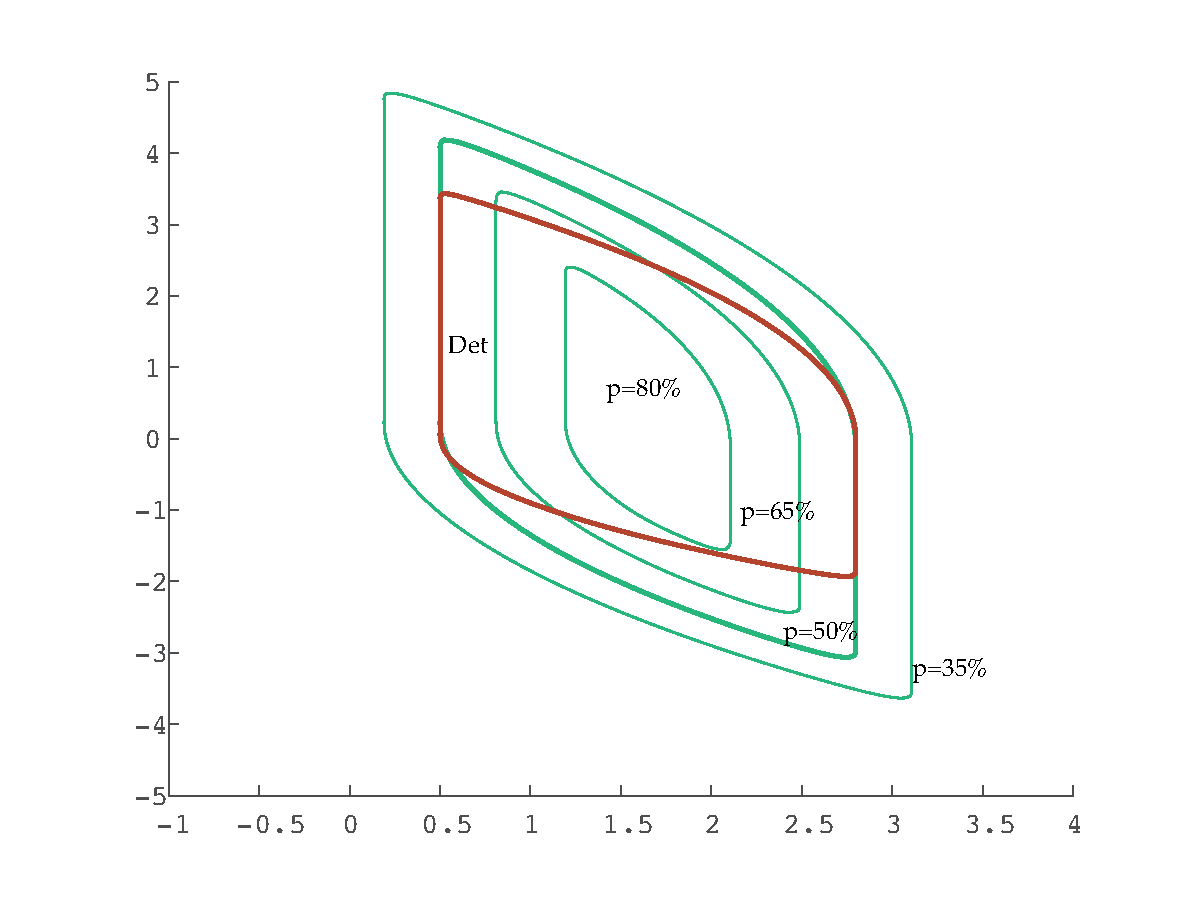
\includegraphics[width=0.9\textwidth]{safetyCompareLabel.eps}
  \caption{Probabilistic Safety Level Sets and Deterministic Safe Set}
  \label{fig:ResultLevels}
\end{figure}

Note that the certain safe set is completely enclosed by the 50\% safe sublevel set, meaning the safe set is guaranteed to have better odds at staying within the safe set.
Unfortunately, the safe set is not completely enclosed by any of the larger probability safe sets (which contradicts theory).
Theoretically, the safe set should have greater than 95\% safety since it's disturbance is bound within $2\sigma$ of the mean.

Further investigation is needed to clarify this phenomenon.

\section{Conclusion}
Stochastic reachability was sucessfully calculated for an application of interest assuming additive white noise.
Many lessons were learnt about the fundamentals of reachability as well as techniques for dealing with stochastic differential equations.
By investigating a variant of reachability, the derivations conducted in class for deterministic reachability had to be re-examined closely and re-derived tracking the addition of white noise all along the way.
This formed an excellent introduction to reachability and forced me to truly grapple with the concepts that make it work.
In the end I discovered that this mathematical problem had already been investigated by Ian Mitchell \cite{MitchellToolbox}, but I learned a lot along the way.
I also hope that this project can illuminate the usefulness of examining reachability in this manner, and revive stochastic reachability investigation in our lab.

  \bibliographystyle{plain}
  \bibliography{BitsAndPieces/primary_cite}

\end{document}
